\documentclass{article}
\usepackage[svgnames]{xcolor}
\usepackage[utf8]{inputenc}
\usepackage{float}
\usepackage{fullpage} % Package to use full page
\usepackage{parskip} % Package to tweak paragraph skipping
\usepackage{tikz} % Package for drawing
\usepackage{amsmath}
\usepackage{hyperref}
\hypersetup{
    colorlinks=true,
    linkcolor=purple,
    filecolor=magenta,      
    urlcolor=pink,
}
\usepackage{amssymb}
\usepackage{bm}
\usepackage{framed}
\usepackage{amsthm}
\usepackage{listings}
\usepackage{biblatex}

\lstset{language=R,
    basicstyle=\small\ttfamily,
    stringstyle=\color{DarkGreen},
    otherkeywords={0,1,2,3,4,5,6,7,8,9},
    morekeywords={TRUE,FALSE},
    deletekeywords={data,frame,length,as,character},
    keywordstyle=\color{blue},
    commentstyle=\color{DarkGreen},
}

\addbibresource{glm-exercises.bib}

\newenvironment{lyxcode}
	{\par\begin{list}{}{
		\setlength{\rightmargin}{\leftmargin}
		\setlength{\listparindent}{0pt}% needed for AMS classes
		\raggedright
		\setlength{\itemsep}{0pt}
		\setlength{\parsep}{0pt}
		\normalfont\ttfamily}%
	 \item[]}
	{\end{list}}


\newcommand\independent{\protect\mathpalette{\protect\independenT}{\perp}}
\def\independenT#1#2{\mathrel{\rlap{$#1#2$}\mkern2mu{#1#2}}}

\newcommand{\E}{\mathrm{E}}
\newcommand{\Var}{\mathrm{Var}}
\newcommand{\Cov}{\mathrm{Cov}}
\newcommand{\Cor}{\mathrm{Cor}}

% vertical line in {bmatrix}
\makeatletter
\renewcommand*\env@matrix[1][*\c@MaxMatrixCols c]{%
 \hskip -\arraycolsep
 \let\@ifnextchar\new@ifnextchar
 \array{#1}}
\makeatother

\title{Exercises in Generalized Linear Models \\ \textbf{Week 41}}
\author{Vinnie Ko, Jonas Moss, and Ørnulf Borgan}
\date{Fall 2020}

\begin{document}
\maketitle
Exercises for the course \href{https://www.uio.no/studier/emner/matnat/math/STK3100/}{STK3100/STK4100: Introduction to Generalized Linear Models} at the University of Oslo, fall 2020. The exercises are from the textbook Alan Agresti: \textit{Foundations of Linear and Generalized Linear Models}. Wiley, 2015. ISBN: 978-1-118-73003-4. The additional exercises are available \href{https://www.uio.no/studier/emner/matnat/math/STK3100/h20/oppgaver.html}{online}. Exercises exclusively nvolving \texttt{R} are not covered.
\section*{Additional Exercise 8}
\subsection*{(a)}
The density can be written as
\begin{align*}
f(y,\pi) & = \pi(1-\pi)^{y},  \\
         & = \exp\left[y \log(1-\pi) + \log\pi\right].
\end{align*}
And we obtain $\theta = \log(1-\pi)$, $\pi = 1-e^{\theta}$, $b(\theta) = -\log\left(1-e^{\theta}\right)$, $a(\phi) = 1$, $c(y,\phi) = 0$.

\subsection*{(b)}
This density can be written
\begin{align*}
f(y,\pi) & = \binom{y+r-1}{r-1}\pi^{r}(1-\pi)^{y} \\ 
         & = \exp\left[y \log(1-\pi) + r\log\pi + \log\binom{y+r-1}{r-1}\right]
\end{align*}
So, $\theta = \log(1-\pi)$, $\pi = 1 -e^{\theta}$ $b(\theta) =-r\log\left(1-e^{\theta}\right)$, $a(\phi) = 1$, $c(y,\phi) = \log\binom{y+r-1}{r-1}$.\\

\subsection*{(c)}
Using the known formula for the expectation and variance, we obtain
\begin{align*}
\E[Y] &= b'(\theta) = r\frac{e^{\theta}}{1-e^{\theta}} = r\left(\frac{1}{\pi}-1\right)\\ \intertext{and}
\Var(Y) &= b''(\theta) a(\phi) = r\frac{e^{\theta}}{\left(1-e^{\theta}\right)^2} = \frac{r}{\pi}\left(\frac{1}{\pi}-1\right).
\end{align*}
\section*{Exercise 4.13}
\subsection*{(i)}
From p.135 of the book, we have that the Pearson chi-squared statistic is defined as $X^{2} = \sum_{i=1}^{n} \frac{(y_{i} - \widehat{\mu}_{i})^{2}}{\Var(Y_{i})}$. Further, it's given that $y_{i} \sim N(\mu_{i},\sigma^{2})$. So, $$X^{2} = \frac{\sum_{i=1}^{n}(y_{i} - \widehat{\mu}_{i})^{2}}{\sigma^{2}} \sim \chi_{n-p}^{2}.$$
The deviance is
\begin{align*}
D(\bm{y},\widehat{\bm{\mu}}) &= -2\left(L\left(\widehat{\bm{\mu}},\bm{y}\right) - L\left(\bm{y},\bm{y}\right)\right),\\
&= -2\left(-\frac{n}{2}\log(2\pi) -n\log\sigma - \frac{1}{2\sigma^{2}}\sum_{i=1}^{n}(y_{i} - \widehat{\mu}_{i})^{2} -\left(-\frac{n}{2}\log(2\pi) -n\log\sigma\right)\right),\\
&= \frac{1}{\sigma^{2}}\sum_{i=1}^{n}(y_{i} - \widehat{\mu}_{i})^{2}.
\end{align*}
So the Pearson chi-squared statistic is the same as the deviance.\\

\subsection*{(ii)}
\begin{align*}
D(\bm{y},\widehat{\bm{\mu}}_{0}) - D(\bm{y},\widehat{\bm{\mu}}_{1}) &= -2\left(L\left(\widehat{\bm{\mu}}_{0},\bm{y}\right) - L\left(\widehat{\bm{\mu}}_{1},\bm{y}\right)\right)\\
&= -2\left(-\frac{1}{2\sigma^{2}}\sum_{i=1}^{n}(y_{i} - \widehat{\mu}_{0,i})^{2} +\frac{1}{2\sigma^{2}}\sum_{i=1}^{n}(y_{i} - \widehat{\mu}_{1,i})^{2}\right)\\
&= \frac{1}{\sigma^{2}}\sum_{i=1}^{n}\left[(y_{i} - \widehat{\mu}_{0,i})^{2} -(y_{i} - \widehat{\mu}_{1,i})^{2}\right]\\
\end{align*}

\section*{Exercise 4.14}
The likelihood equation of GLM is $\frac{\partial L(\bm{\beta})}{\partial \beta_{j}} = \sum_{i=1}^{n}\frac{(y_{i}-\mu_{i})x_{i,j}}{\Var(Y_{i})}\frac{\partial \mu_{i}}{\partial \eta_{i}} = 0$ (p.124 of the book).\\
For the intercept. this becomes 
$\frac{\partial L(\bm{\beta})}{\partial \beta_{0}} = \sum_{i=1}^{n}\frac{(y_{i}-\mu_{i})}{\Var(Y_{i})}\frac{\partial \mu_{i}}{\partial \eta_{i}} = 0$.

The canonical link function $g$ is the function satisfying $\theta = g\left(\E[Y] \right)$. (p. 123 of the book).\\
So, $\frac{\partial \mu_{i}}{\partial \eta_{i}} = \frac{\partial \mu_{i}}{\partial \theta_{i}} = \frac{\partial b'(\theta_{i})}{\partial \theta_{i}} = b''(\theta_{i})$. Further, we know $\Var(Y_{i}) = b''(\theta_{i})a(\phi)$.\\
Thus,
\begin{align*}
\frac{\partial L(\bm{\beta})}{\partial \beta_{0}} &= \sum_{i=1}^{n}\frac{(y_{i}-\mu_{i})}{\Var(Y_{i})}\frac{\partial \mu_{i}}{\partial \eta_{i}}\\
&= \sum_{i=1}^{n}(y_{i}-\mu_{i})\frac{1}{a(\phi)}\\
&= 0
\end{align*}
In most cases $a(\phi)$ doesn't depend on the data. In that case, 
\begin{align*}
\frac{\partial L(\bm{\beta})}{\partial \beta_{0}} = \frac{1}{a(\phi)}\sum_{i=1}^{n}(y_{i}-\mu_{i}) = 0.
\end{align*}
So, $\sum_{i=1}^{n}y_{i} = \sum_{i=1}^{n}\widehat{\mu}_{i}$ and this equality doesn't necessarily hold for a GLM with non-canonical function.\\
Obviously, when there is no $\beta_{0}$ for a GLM with canonical link function, we can't derive this equality.
\section*{Exercise 4.16}
\textbf{Note:} I use the binomial distribution as defined in p. 122 of the book. This implies that $y_{i}$ is a proportion of success, instead of a number of success.

\subsection*{(a)}
The pmf of binomial distribution is
\begin{align*}
f(y_{i}) &= \binom{n_{i}}{n_{i}y_{i}} \pi_{i}^{n_{i}y_{i}} (1-\pi_{i})^{n_{i}-n_{i}y_{i}}\\
&= \exp\left[\frac{\theta_{i}y_{i} -\log\left(1+e^{\theta_{i}}\right)}{\frac{1}{n_{i}}} + \log\binom{n_{i}}{n_{i}y_{i}}\right]\\
&= \exp\left[\frac{\theta_{i}y_{i} -b(\theta_{i})}{a(\phi)} + c(y_{i},\phi)\right]
\end{align*}
where $\theta_{i} = \log\left(\frac{\pi_{i}}{1-\pi_{i}}\right)$, $\pi_{i} = \frac{e^{\theta_{i}}}{1+e^{\theta_{i}}}$, $b(\theta_{i}) = \log\left(1+e^{\theta_{i}}\right) = -\log\left(1-\pi_{i}\right)$, $c(y_{i}) = \log\binom{n_{i}}{n_{i}y_{i}}$, $a(\phi) = \frac{1}{n_{i}}$.\\
Since $a(\phi) = \frac{1}{n_{i}}$, $w_{i} = n_{i}$ (p.121 of the book) and we have
\begin{align*}
d_{i} &= 2w_{i}\left[y_{i}\left(\widetilde{\theta}_{i} - \widehat{\theta}_{i}\right) -b\left(\widetilde{\theta}_{i}\right) + b\left(\widehat{\theta}_{i}\right)\right]\\
&= 2n_{i}\left[y_{i}\left(\log\left(\frac{y_{i}}{1-y_{i}}\right) -  \log\left(\frac{\widehat{\pi}_{i}}{1-\widehat{\pi}_{i}}\right)\right) +\log\left(1-y_{i}\right) -\log\left(1-\widehat{\pi}_{i}\right)\right]\\
&= 2n_{i}\left[y_{i}\log y_{i} - y_{i}\log (1-y_{i}) - y_{i}\log\widehat{\pi}_{i} +y_{i}\log(1-\widehat{\pi}_{i}) +\log\left(1-y_{i}\right) -\log\left(1-\widehat{\pi}_{i}\right)\right]\\
&= 2n_{i}\left[y_{i}\log \frac{y_{i}}{\widehat{\pi}_{i}} +(1-y_{i})\log\left(\frac{1-y_{i}}{1-\widehat{\pi}_{i}}\right)\right]\\
&= 2\left[n_{i}y_{i}\log \frac{y_{i}}{\widehat{\pi}_{i}} +n_{i}(1-y_{i})\log\left(\frac{1-y_{i}}{1-\widehat{\pi}_{i}}\right)\right].
\end{align*}

\subsection*{(b)}
The pmf of Poisson distribution is
\begin{align*}
f(y_{i}) &= \frac{\mu_{i}^{y_{i}}}{y_{i}!}e^{-\mu_{i}}\\
&= \exp\left[y_{i}\log\mu_{i} -\mu_{i} -\log y_{i}!\right]\\
&= \exp\left[\frac{\theta_{i}y_{i} -b(\theta_{i})}{a(\phi)} + c(y_{i},\phi)\right]
\end{align*}
where $\theta_{i} = \log\mu_{i}$, $b(\theta_{i}) = e^{\theta_{i}} = \mu_{i}$, $c(y_{i}) = -\log y_{i}!$, $a(\phi) = 1$, $w_{i} = 1$.\\
Thus, we have
\begin{align*}
d_{i} &= 2w_{i}\left[y_{i}\left(\widetilde{\theta}_{i} - \widehat{\theta}_{i}\right) -b\left(\widetilde{\theta}_{i}\right) + b\left(\widehat{\theta}_{i}\right)\right]\\
&= 2\left[y_{i}\left(\log y_{i} -\log\widehat{\mu}_{i}\right) -y_{i} +\widehat{\mu}_{i}\right]\\
&= 2\left[y_{i}\log\left(\frac{y_{i}}{\widehat{\mu}_{i}}\right) -y_{i} +\widehat{\mu}_{i}\right].
\end{align*}
This matches the expression in p.133 of the book.
\vspace{\baselineskip}
\section*{Exercise 4.19}
\subsection*{(a)}
For $\beta^{(0)}$ that is close to $\widehat{\beta}$, we can use first order Taylor approximation
\begin{align*}
0 = L'(\widehat{\beta}) = L'(\beta^{(0)}) + \left(\widehat{\beta}-\beta^{(0)}\right)L''(\beta^{(0)}) + o_p (n^{-\frac{1}{2}}).
\end{align*}
We can rewrite this as
\begin{align*}
\widehat{\beta} \approx \beta^{(0)} - \frac{L'(\beta^{(0)})}{L''(\beta^{(0)})}.
\end{align*}
Approximating $\widehat{\beta}$ by $\beta^{(1)}$ gives us
\begin{align*}
\beta^{(1)} = \beta^{(0)} - \frac{L'(\beta^{(0)})}{L''(\beta^{(0)})}.
\end{align*}
\subsection*{(b)}
By generalizing the result from a), we have
\begin{align*}
\beta^{(t+1)} = \beta^{(t)} - \frac{L'(\beta^{(t)})}{L''(\beta^{(t)})}.
\end{align*}

\section*{Exercise 4.20}
The pmf of Poisson distribution is
\begin{align*}
f(y) = \frac{\mu^{y}}{y!}e^{-\mu}
\end{align*}
So,
\begin{align*}
L(\bm{y}) &= \log\mu\sum_{i=1}^{n}y_{i} - n\mu -\sum_{i}^{n}\log y_{i}!\\
\frac{\partial L(\bm{y})}{\partial \mu} &= \frac{1}{\mu}\sum_{i=1}^{n}y_{i} -n = -n +\frac{n\overline{y}}{\mu}\\
H &= \frac{\partial^{2} L(\bm{y})}{\partial \mu^{2}} = -\frac{n\overline{y}}{\mu^{2}}\\
\mathcal{J} &= \E\left[-\frac{\partial^{2} L(\bm{Y})}{\partial \mu^{2}}\right] = \frac{n}{\mu^{2}}\E\left[\overline{Y}\right] = \frac{n}{\mu}.
\end{align*}

Fisher scoring gives
\begin{align*}
\mu^{(t+1)} = \mu^{(t)} + \left(\mathcal{J}^{(t)}\right)^{-1}u^{(t)} = \mu^{(t)} + \frac{\mu^{(t)}}{n}\left(-n +\frac{n\overline{y}}{\mu^{(t)}}\right) = \overline{y}.
\end{align*}

Newton-Raphson gives
\begin{align*}
\mu^{(t+1)} = \mu^{(t)} + \left(H^{(t)}\right)^{-1}u^{(t)} = \mu^{(t)} -\frac{\left(\mu^{(t)}\right)^{2}}{n\overline{y}}\left(-n +\frac{n\overline{y}}{\mu^{(t)}}\right) = \mu^{(t)}\left(2 - \frac{\mu^{(t)}}{\overline{y}}\right).
\end{align*}
Note that if $\mu^{(t)} = \overline{y}$, then $\mu^{(t+1)} = \overline{y}$.
\section*{Exercise 5.13}
We do this exercise with unstandardized residuals. The solution and intuition is similar for the other residuals, but requires more calculations to find the theoretical residual lines.
\begin{lstlisting}[language=R]
# Parameters for the problem.

n = 100
min = 0
max = 100

# Make the theoretical residuals.

x = seq(min, max, by = 0.1)
y = plogis(-2.0 + 0.04 * x)

plot(
  x = x, 
  y = -y, 
  type = "l", 
  ylim = c(-1, 1), 
  main = "Residuals",
  ylab = "Residuals")

lines(x = x, y = 1 - y)

# Simulate some values.

set.seed(313) # Reproducibility.
x = runif(n = n, min = min, max = max)
y = -2.0 + 0.04 * x + rlogis(n) >= 0
model = glm(y ~ x, family = binomial(link = "logit"))

# Add to plot.
col = c("red", "blue")[y + 1]
points(x, y - fitted(model), col = col, pch = 20)
\end{lstlisting}

\begin{center}
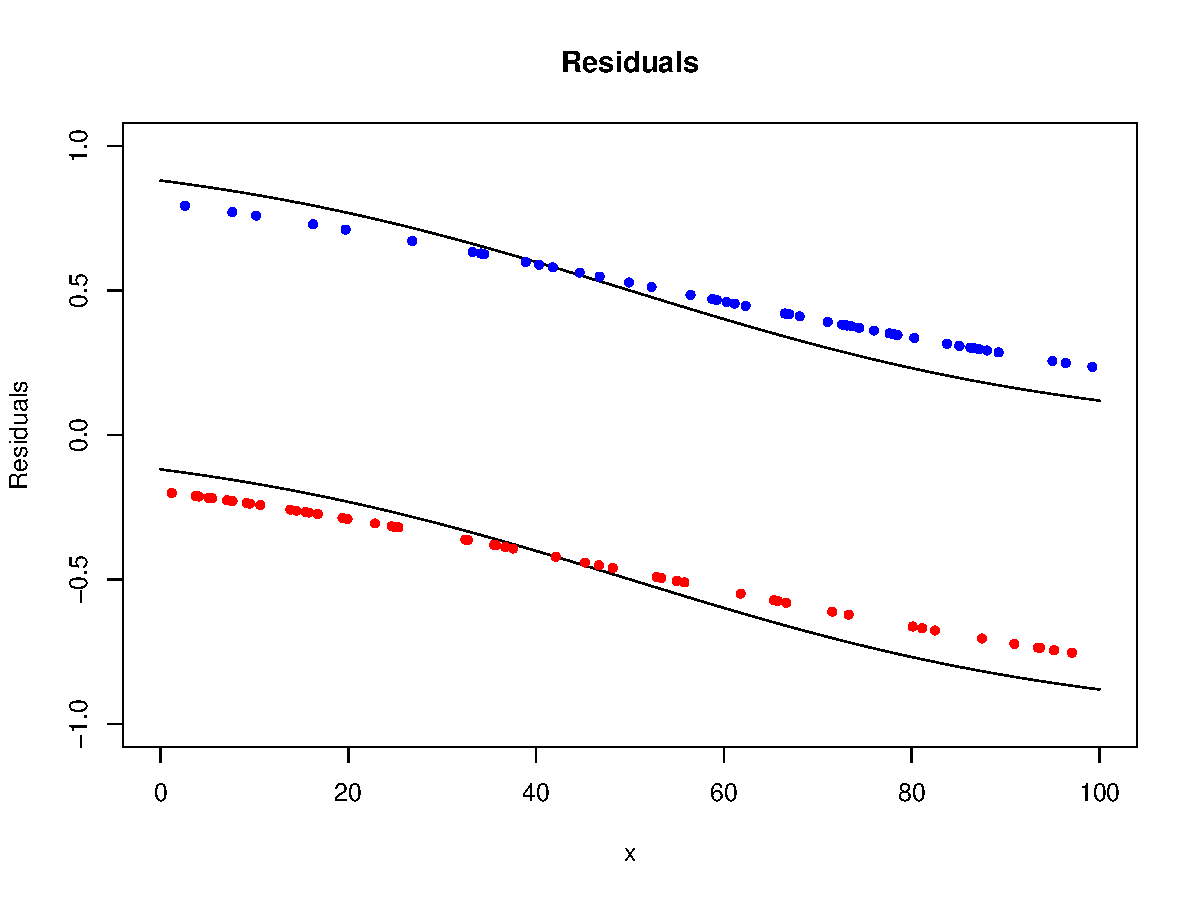
\includegraphics[scale=0.7]{figures/exercise-5.13.pdf}
\end{center}
\section*{Exercise 5.14}
\textbf{Note:} I use the binomial distribution as defined in p.122 of the book. This implies that $y_{i}$ is a proportion of success, instead of a number of success.\\

The binomial pmf with a common $\pi$ is
\begin{align*}
f(y_{i}) &= \binom{n_{i}}{n_{i}y_{i}} \pi^{n_{i}y_{i}} (1-\pi)^{n_{i}-n_{i}y_{i}}
\end{align*}

Then, the log-likelihood is
\begin{align*}
L(\pi) = \sum_{i=1}^{N} \left[\log\binom{n_{i}}{n_{i}y_i} + n_{i}y_{i}\log\pi + (n_{i} -n_{i}y_{i})\log(1-\pi)\right].
\end{align*}
By solving
\begin{align*}
\frac{\partial L(\pi)}{\partial \pi} =  \frac{1}{\pi}\sum_{i=1}^{N}n_{i}y_{i} -\frac{1}{1-\pi}\sum_{i=1}^{N}(n_{i}-n_{i}y_{i}) = 0
\end{align*}
\begin{align*}
(1-\pi)\sum_{i=1}^{N}n_{i}y_{i}  = \pi\sum_{i=1}^{N}(n_{i}-n_{i}y_{i})
\end{align*}
we obtain
\begin{align*}
\widehat{\pi} = \frac{\sum_{i=1}^{N}n_{i}y_{i}}{\sum_{i=1}^{N}n_{i}}.
\end{align*}

The Pearson chi-squared statistic (p. 135 of the book) is
\begin{align*}
X^{2} &= \sum_{i=1}^{N} \frac{(y_{i} - \widehat{\pi})^{2}}{\Var(Y_{i})}\\
&= \sum_{i=1}^{N} \frac{(y_{i} - \widehat{\pi})^{2}}{\widehat{\pi}(1-\widehat{\pi})/n_{i}}
\end{align*}
When all $n_{i} = 1$, we obtain $\widehat{\pi} = \frac{\sum_{i=1}^{N}n_{i}y_{i}}{\sum_{i=1}^{N}n_{i}} = \frac{\sum_{i=1}^{N}y_{i}}{N}$ and
\begin{align*}
X^{2} &= \sum_{i=1}^{N} \frac{(y_{i} - \widehat{\pi})^{2}}{\Var(Y_{i})}\\
&= \frac{1}{\widehat{\pi}(1-\widehat{\pi})}\sum_{i=1}^{N}(y_{i} - \widehat{\pi})^{2}\\
&= \frac{1}{\widehat{\pi}(1-\widehat{\pi})}\sum_{i=1}^{N}(y_{i}^{2} -2\widehat{\pi}y_{i} + \widehat{\pi}^{2})\\
&= \frac{1}{\widehat{\pi}(1-\widehat{\pi})}\left(\sum_{i=1}^{N}y_{i} -2\widehat{\pi}\sum_{i=1}^{N}y_{i} +N\widehat{\pi}^{2}\right)\\
&= \frac{1}{\widehat{\pi}(1-\widehat{\pi})}\left(N\widehat{\pi} -2\widehat{\pi}N\widehat{\pi} +N\widehat{\pi}^{2}\right)\\
&= \frac{1}{\widehat{\pi}(1-\widehat{\pi})}N\widehat{\pi}\left(1 -\widehat{\pi}\right)\\
&= N.
\end{align*}

\section*{Exam 2015 Problem 1}
\subsection*{(a)}
The probability mass function of a binomially distributed variable
is
\begin{eqnarray*}
f(y;\pi) & = & \binom{n}{y}\pi^{y}(1-\pi)^{n-y},\\
 & = & {\binom{n}{y}}\exp\left(y\log\left[\frac{\pi}{1-\pi}\right]+n\log(1-\pi)\right).
\end{eqnarray*}
From this representation we can read off, using the form
\[
\exp\left[\frac{y\theta-b(\theta)}{a(\phi)}+c(y,\phi)\right],
\]
that
\begin{eqnarray*}
\theta & = & \log\left[\frac{\pi}{1-\pi}\right],\\
a(\theta) & = & -n\log(1-\pi),\\
\phi & = & 1,\\
c(y,\phi) & = & \log{\binom{n}{y}}.
\end{eqnarray*}
The link function connects the linear combination $\beta^{T}X$ to
the parameter $\theta$ using the relation $g(\theta)=\beta^{T}X$.

\subsection*{(b)}
The likelihood in a generalized linear model is
\[
L(\theta;y)=\prod_{i=1}^{n}\exp\left[\frac{y_{i}\theta_{i}-b(\theta_{i})}{a(\phi)}+c(y_{i},\phi)\right].
\]
If $\check{\theta}$ and $\hat{\theta}$ are the fitted parameter
vectors in a saturated and another model, the deviance is
\begin{eqnarray*}
\Delta & = & 2\log L(\check{\theta};y)-2\log L(\hat{\theta},y),\\
 & = & 2\sum_{i=1}^{n}\left[\frac{y_{i}\check{\theta}_{i}-a(\check{\theta}_{i})}{\phi}-\frac{y_{i}\hat{\theta}_{i}-a(\hat{\theta}_{i})}{\phi}\right],\\
 & = & 2\sum_{i=1}^{n}\left[y_{i}(\check{\theta}_{i}-\hat{\theta}_{i})-b(\check{\theta}_{i})+b(\hat{\theta}_{i})\right].
\end{eqnarray*}
For the binomial distribution we have
\begin{eqnarray*}
\check{\theta}_{i} & = & \log(y_{i}/(n_{i}-y_{i}),\\
\hat{\theta}_{i} & = & \log(\hat{\mu}_{i}/(n_{i}-\hat{\mu}_{i}),
\end{eqnarray*}
and 
\begin{eqnarray*}
b(\check{\theta}_{i}) & = & -n_{i}\log(1-y_{i}/n_{i}),\\
b(\hat{\theta}_{i}) & = & -n_{i}\log(1-\hat{\mu}_{i}/n_{i}).
\end{eqnarray*}
Plugging this into the expression for the deviance above yields
\[
\Delta=2\sum_{i=1}^{n}[y_{i}\log(y_{i}/\hat{\mu}_{i})+(n_{i}-y_{i})\log[(n_{i}-y_{i})/(n_{i}-\hat{\mu}_{i})].
\]
The deviance is primarily used do significance testing with nested
models.

\section*{Exam 2017 Problem 2}

\subsection*{(a)}
The variable $Y$ has a Poisson distribution, with probability mass
function
\[
P(Y=y;\lambda)=\frac{\lambda^{y}}{y!}e^{-\lambda},\quad y=0,1,2,\ldots.
\]
We want to write probability on the canonical form
\[
\exp\left[\frac{y\theta-b(\theta)}{a(\phi)}+c(y,\phi)\right].
\]
This is easily done using exponentiation and logarithms:
\[
P(Y=y;\lambda)=\frac{\lambda^{y}}{y!}e^{-\lambda}=e^{y\log\lambda-\lambda\log(y!)}.
\]
Now we identify the terms of of the canonical form:
\begin{eqnarray*}
\theta & = & \log(\lambda),\\
b(\theta) & = & \lambda=e^{\theta},\\
a(\phi) & = & 1,\\
c(y,\phi) & = & -\log(y!).
\end{eqnarray*}

\subsection*{(b)}
A generalized model is a regression model where
\[
Y_{i}\mid X_{i}\sim f(g^{-1}(X_{i}^{T}\beta),\phi)
\]
for some density $f(\mu,\phi)$ in the exponential dispersion family
with mean parameter $\mu$ and dispersion parameter $\phi$. The function
$g$ is strictly increasing, differentiable, and called the \emph{link
function}. (A strictly increasing function almost everywhere differentiable,
by the way.) It connects the mean to the $X_{i}^{T}\beta$ by $g(\mu)=X_{i}^{T}\beta$.
Sometimes the model is formulated in terms of the canonical parameter
$\theta_{i}$ where $\mu_{i}=b'(\theta_{i})$ in the formulation above.
\subsection*{(c)}
Using the result from (a), we find the log-likelihood is
\[
L(\mu,y)=\sum_{i=1}^{n}\{y_{i}\log\mu_{i}-\mu_{i}-\log(y_{i}!)\}.
\]
\subsection*{(d)}
For a saturated model there are no restrictions on the expected values,
so there is a separately fitted parameter $\mu_{i}$ for each observation
$y_{i}$.

The log-likelihood attains its maximum when
\[
\frac{\partial}{\partial\mu_{i}}L(\mu;y)=0,\quad i=1,\ldots,n.
\]
Now we have
\[
\frac{\partial}{\partial\mu_{i}}L(\mu;y)=\frac{y_{i}}{\mu_{i}}-1,
\]
so the log-likelihood takes its maximal value when $y_{i}=\mu_{i}$,
and the maximal value of the log-likelihood is
\[
L(y;y)=\sum_{i=1}^{n}\{y_{i}\log y_{i}-y_{i}-\log(y_{i}!)\}.
\]
\subsection*{(e)}
The deviance is defined as
\[
\Delta=D(y;\mu)=2\left(L(\check{\theta};y)-L(\hat{\theta};y)\right),
\]
where $\hat{\theta}$ is the maximum likelihood estimator of our model
and $\check{\theta}$ is the maximum likelihood estimator of the saturated
model. In our Poisson case, the deviance is
\[
2\sum_{i=1}^{n}\{y_{i}\log y_{i}-y_{i}-\log(y_{i}!)\}-2\sum_{i=1}^{n}\{y_{i}\log\hat{\mu}_{i}-\hat{\mu}_{i}-\log(y_{i}!)\},
\]
which equals
\[
2\sum_{i=1}^{n}\left\{ y_{i}\log(y_{i}/\hat{\mu}_{i})-y_{i}+\hat{\mu}_{i}\right\} .
\]
The deviance is used for carrying out significance tests for nested
models, as $\Delta\sim\chi_{n-p}^{2}$ asymptotically, where $p$
is the number of fitted parameters in the non-saturated model.

\printbibliography
\end{document}
